%================================================================
%                           N O T E S
%                           ---------
%
%                           ---------
%-----------------------------------------------------------------
%                       INTRODUCTION
%-----------------------------------------------------------------
\section{Introduction}
We now want to consider what happens inside a cylinder of different density to the outside medium. We consider our same plane wave inciding on this cylinder, see \figref{fig:problem_2}. The goal in this section is to find an expression for the velocity field over the entire domain. \par

We can divide this problem into two domains: the wave field inside the cylinder and outside the cylinder. Similar the previous problem we have
\begin{equation}
  \Phi_{tot} = \Phi_{1} + \Phi_{2} + \Phi_{in}
\end{equation}
where $\Phi_{1}$ and $\Phi_{2}$ are the potential fields for the outside and inside velocity fields respectively.

We already have an expression for the incident field from the previous chapter:
\begin{gather}
  \Phi_{in} = e^{- i(\vec{k} \cdot \vec{x})}.
\end{gather}

Physically, we still expect the wave outside the cylinder to dissipate and satisfy the Sommerfeld Radiation Condition. Hence, the solution from the previous chapter still applies, except the constant $B_n$ will be determined by the boundary condition specific for this problem. This is discussed later on in this chapter. So we have
\begin{equation}
  \Phi_1 = \sum^\infty_{n=0} \epsilon_n i^n B_1 H_n(kr) \cos(n\theta).
\end{equation}

All that is left now is to find $\Phi_2$.

\begin{figure} \centering
  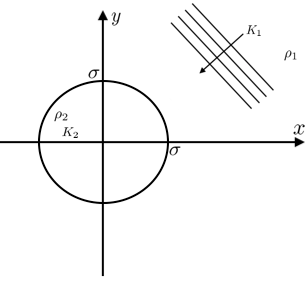
\includegraphics[width=6cm]{../figures/prob2_sketch.png}
  \caption{Plane wave travelling through medium 1 incident on a cylinder (medium 2)}\label{fig:problem_2}
\end{figure}

\begin{figure} \centering
  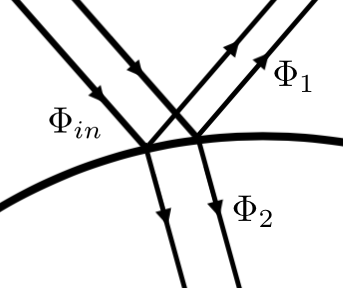
\includegraphics[width=4cm]{../figures/transmission_diagram}
  \caption{Reflection and transmission of the incident wave}
\end{figure}

%---------------------------------------------------------------------
%
%             Potential field inside the cylinder
%
%---------------------------------------------------------------------
\section{Solution inside the cylinder}

To recover an expression for the field outside the cylinder in the previous chapter we first of all make two assumtptions: that $\Phi$ is separabale and that it satisfies the Helmholtz equation. In Proposition \ref{propn:scattered_field_differential_equations} we show that this leads to two independent differential equations, one for $\Theta(\theta)$ and one for $R(r)$. The solution for $\Theta(\theta)$ still applies, since the only addditional assumption there is that the function must be $2 \pi$ periodic, which is clearly the case inside the cylinder too.

We are then left with the bessel differential equation to solve for $R(r)$. This problem is therefore a reformulation of the one we solved previously. Where before we had a wave that was well defined as as $r\rightarrow\infty$, we now have a wave which must be well defined as $r\rightarrow 0$.

We can make use of the propositions in \ssref{ss:limits_of_bessel_functions}, where we consider the behaviour of Bessel equations of different kind as $r\rightarrow\infty$ and $r\rightarrow 0$. Only Bessel functions of the first kind are well defined as $r\rightarrow 0$ for $n\in \bb{Z}$.

\begin{propn}
\begin{equation}
  \Phi_2 = \sum_{n=0}^{\infty} \epsilon_n i^n B_2 J_n(kr) \cos(n\theta)
\end{equation}
\end{propn}
\begin{proof}
  Immediate.
\end{proof}

We can now apply boundary conditions to find the constants we are missing.
%---------------------------------------------------------------------
%
%                 BOUNDARY CONDTION
%
%---------------------------------------------------------------------
\section{Boundary conditions}

We consider the boundary conditions for the reflection of a sound wave at the boundary or two media, which are known \parencite[$\S 11$]{sen14acoustics} to be
\begin{enumerate}[label=(\roman*)]
  \item velocity normal to the boundary must be continuous, and
  \item pressure must be continuous.
\end{enumerate}

\begin{propn} The first boundary condition gives us the following relationship between $B_1$ and $B_2$
  \[ \rho_1 J_n(k\sigma) + \rho_1 B_1 H_n(k\sigma) = \rho_2 B_2 J_n (k\sigma) \].
\end{propn}
\begin{proof}
  In Chapter 1 we derived the linear wave equation from the governing equations using perturbation theory. Going back now to \ssref{ss:perturbation}, we have the modified Momentum equation \eqref{eq:perturbed_momentum}:
  \begin{equation*}
    \rho \partialfrac{\vec{u}}{t} + \nabla p = 0.
  \end{equation*}

  We also showed in Chapter 1 that we can write $\vec{u} = \nabla \phi$, and that for $\phi = \Re[\Phi(\vec{x})T(t)]$, $T(t)=e^{-i\omega t}$, so we have
  \begin{gather*}
    \frac{dT}{dt} = - i\omega T(t), \\
    \partialfrac{\vec{u}}{t} = \nabla \Re\left[\Phi \frac{dT}{dt} \right]
    = -i \omega \nabla \Re\left[ \Phi \right] = -i \omega \nabla \phi.
  \end{gather*}

  This means that we have a linear relationship between $\phi$, the velocity field potential and $p$, the pressure field.
  \begin{align*}
    -i \omega \rho \nabla \phi &= - \nabla p \\
    \nabla (i \omega \rho \phi) &= \nabla p \\
    i \omega \rho \phi &= p \\
    p &\propto \phi
  \end{align*}

  The boundary condition tells us that at the boundary $r=\sigma$, $p_1 = p_2$
  \begin{gather*}
    \Leftrightarrow \rho_1 \left(\phi_{1} + \phi_{incident} \right) = \rho_2 \phi_{2} \\
    \Leftrightarrow \rho_1 \left(\Re[ \Phi_1 T(t) ]  + \Re[\Phi_{in}T(t)] \right) = \rho_2 \Re[\Phi_{2}T(t)]\\
    \Leftrightarrow \rho_1 \left(\Phi_1  + \Phi_{in} \right) = \rho_2 \Phi_{2}
  \end{gather*}

  So we have
  \[ \rho_1 J_n(k\sigma) + \rho_1 B_1 H_n(k\sigma) = \rho_2 B_2 J_n (k\sigma) \]
  as required.
\end{proof}

\begin{propn} The second boundary condition gives us the following relationship between $B_1$ and $B_2$
  \[ B_2 J'n(k\sigma) = B_1 H'_n(k\sigma) + J'n(k\sigma)\].
\end{propn}
\begin{proof}
  The second boundary condition tells us that
  \begin{equation*}
    \partialfrac{\Phi_2}{n} = \partialfrac{\Phi_1}{n} + \partialfrac{\Phi_{in}}{n}  \text{ at } r=\sigma,
  \end{equation*}
  hence,
  \begin{align*}
    B_2J'_n(k\sigma) = B_1 H'_n(k\sigma) + J'n(k\sigma)
  \end{align*}
  as required.
\end{proof}

\begin{propn}
  \begin{gather*}
    B_1 = J_n (k\sigma)J'n(k\sigma)\frac{(\rho_2-\rho_1)}{R_1 - R_2}, \text{ and}\\
    B_2 = \frac{\rho_2R_1- \rho_1 R_2}{\rho_2(R_1 - R_2)}
  \end{gather*}
\end{propn}
\begin{proof}
  We have
  \begin{align*}
  \text{(BC1)  }& \rho_1 J_n(k\sigma) + \rho_1 B_1 H_n(k\sigma) = \rho_2 B_2 J_n (k\sigma), \text{ and}\\
  \text{(BC2)  }& B_2 J'n(k\sigma) = B_1 H'_n(k\sigma) + J'n(k\sigma)
  \end{align*}
  So,
  \begin{align*}
    \text{(BC1)} \Rightarrow B_2 &= \frac{\rho_1 J_n(k\sigma) + \rho_1 B_1 H_n(k\sigma)}{\rho_2 J_n (k\sigma)}, \\
    \text{(BC2)} \Rightarrow B_2 &= \frac{B_1 H'_n(k\sigma) + J'n(k\sigma)}{J'n(k\sigma)}
  \end{align*}
  Finding $B_1$,
  \begin{gather*}
    \frac{\rho_1 J_n(k\sigma) + \rho_1 B_1 H_n(k\sigma)}{\rho_2 J_n (k\sigma)} = \frac{B_1 H'_n(k\sigma) + J'n(k\sigma)}{J'n(k\sigma)} \\
    J'n(k\sigma)(\rho_1 J_n(k\sigma) + \rho_1 B_1 H_n(k\sigma)) = \rho_2 J_n (k\sigma)(B_1 H'_n(k\sigma) + J'n(k\sigma)), \\
    B_1 \left[ \rho_1 J'n(k\sigma) H_n(k\sigma) -  \rho_2 J_n (k\sigma) H'_n(k\sigma) \right] = \rho_2 J_n (k\sigma)J'n(k\sigma) - \rho_1 J'n(k\sigma) J_n(k\sigma) \\
    B_1 = \frac{(\rho_2-\rho_1)J_n (k\sigma)J'n(k\sigma)}{ \rho_1 J'n(k\sigma) H_n(k\sigma) -  \rho_2 J_n (k\sigma) H'_n(k\sigma)}
  \end{gather*}
  and $B_2$,
  \begin{gather*}
    \text{(BC2)} \Rightarrow B_2 = \frac{H'_n(k\sigma)}{J'n(k\sigma)}B_1 + 1
  \end{gather*}
  \begin{align*}
    B_2 &= \frac{H'_n(k\sigma)}{J'n(k\sigma)} \left\{ \frac{(\rho_2-\rho_1)J_n (k\sigma)J'n(k\sigma)}{ \rho_1 J'n(k\sigma) H_n(k\sigma) -  \rho_2 J_n (k\sigma) H'_n(k\sigma)} \right\} + 1 \\
    &= \frac{(\rho_2-\rho_1)J_n (k\sigma)H'_n(k\sigma) + \rho_1 J'n(k\sigma) H_n(k\sigma) -  \rho_2 J_n (k\sigma) H'_n(k\sigma)
    }{
    \rho_1 J'n(k\sigma) H_n(k\sigma) -  \rho_2 J_n (k\sigma) H'_n(k\sigma)} \\
    &= \frac{-\rho_1 J_n (k\sigma)H'_n(k\sigma) + \rho_1 J'n(k\sigma) H_n(k\sigma)}{\rho_1 J'n(k\sigma) H_n(k\sigma) -  \rho_2 J_n (k\sigma) H'_n(k\sigma)}
  \end{align*}
  Notice that there are two values that are common to both expressions: $\rho_1 J'n(k\sigma) H_n(k\sigma)$, and $\rho_2 J_n (k\sigma) H'_n(k\sigma)$. Let the first be $R_1$ and the second $R_2$. Then we have,
  \begin{gather*}
    B_1 = \frac{(\rho_2-\rho_1)J_n (k\sigma)J'n(k\sigma)}{R_1 - R_2} \\
    B_2 = \frac{\rho_1(R_1/\rho_1- R_2/\rho_2)}{R_1 - R_2} = \frac{\rho_2R_1- \rho_1 R_2}{\rho_2(R_1 - R_2)}
  \end{gather*}
  as required.
\end{proof}
